\documentclass{exam}
\usepackage[utf8]{inputenc}
\usepackage{lmodern}
\usepackage{microtype}

% \usepackage[parfill]{parskip}
\usepackage[dvipsnames]{xcolor}
\usepackage{amsmath}
\usepackage{amsfonts}
\usepackage{amsthm}
\usepackage{siunitx}
\DeclareSIUnit\year{yr}
\DeclareSIUnit\foot{ft}
\DeclareSIUnit\litre{\liter}

\usepackage{skull}

\usepackage{pgfplots}
\usepgfplotslibrary{polar}
\pgfplotsset{compat=1.11}
\usepgfplotslibrary{statistics}
\usepackage{graphicx}
\usepackage{sidecap}
\sidecaptionvpos{figure}{c}
\usepackage{float}
\usepackage{gensymb}
\usepackage{tkz-euclide}
\usetkzobj{all}
\usepackage{commath}
\usepackage{hyperref}
\usepackage{enumitem}
\usepackage{wasysym}
\usepackage{multicol}
\usepackage{mathtools}
\usepackage{tcolorbox}
\usepackage{tabularx}
\usepackage[version=4]{mhchem}
\usepackage{changepage}
\usepackage{listings}
\lstset{basicstyle=\ttfamily\linespread{0.8}\small}

\renewcommand*{\thefootnote}{\fnsymbol{footnote}}

\newtheorem*{thm}{Theorem}
\newtheorem*{iden}{Identity}
\newtheorem*{lemma}{Lemma}
\newtheorem{obs}{Observation}
\theoremstyle{definition}
\newtheorem*{defn}{Definition}
\newtheorem*{ex}{Example}
\newtheorem{con}{Construction}
\newtheorem*{alg}{Algorithm}

\newtheoremstyle{break}
  {\topsep}{\topsep}%
  {\itshape}{}%
  {\bfseries}{}%
  {\newline}{}%
\theoremstyle{break}
\newtheorem*{bthm}{Theorem}

% russian integral
\usepackage{scalerel}
\DeclareMathOperator*{\rint}{\scalerel*{\rotatebox{17}{$\!\int\!$}}{\int}}

% \DeclareMathOperator*{\rint}{\int}

\pgfplotsset{vasymptote/.style={
    before end axis/.append code={
        \draw[densely dashed] ({rel axis cs:0,0} -| {axis cs:#1,0})
        -- ({rel axis cs:0,1} -| {axis cs:#1,0});
    }
}}

% \pointsinrightmargin
\boxedpoints
\pointname{}

\newcommand{\questioA}{\question[\texttt{\textbf{\color{Cerulean} A}}]}
\newcommand{\questioM}{\question[\texttt{\textbf{\color{PineGreen} M}}]}
\newcommand{\questioE}{\question[\texttt{\textbf{\color{WildStrawberry} E}}]}
\newcommand{\questioS}{\question[\texttt{\textbf{\color{Goldenrod} S}}]}
\newcommand{\questioO}{\question[\texttt{\textbf{\color{BurntOrange} O}}]}

\newcommand{\parA}{\part[\texttt{\textbf{\color{Cerulean} A}}]}
\newcommand{\parM}{\part[\texttt{\textbf{\color{PineGreen} M}}]}
\newcommand{\parE}{\part[\texttt{\textbf{\color{WildStrawberry} E}}]}
\newcommand{\parS}{\part[\texttt{\textbf{\color{Goldenrod} S}}]}
\newcommand{\parO}{\part[\texttt{\textbf{\color{BurntOrange} O}}]}

\newcommand{\subparA}{\subpart[\texttt{\textbf{\color{Cerulean} A}}]}
\newcommand{\subparM}{\subpart[\texttt{\textbf{\color{PineGreen} M}}]}
\newcommand{\subparE}{\subpart[\texttt{\textbf{\color{WildStrawberry} E}}]}
\newcommand{\subparS}{\subpart[\texttt{\textbf{\color{Goldenrod} S}}]}
\newcommand{\subparO}{\subpart[\texttt{\textbf{\color{BurntOrange} O}}]}

\newcommand{\mainHeader}[2]{\section*{NCEA Level 2 Mathematics\\#1. #2}}
\newcommand{\mainHeaderHw}[2]{\section*{NCEA Level 2 Mathematics (Homework)\\#1. #2}}
\newcommand{\seealso}[1]{\begin{center}\emph{See also #1.}\end{center}}
\newcommand{\drills}[1]{\begin{center}\emph{Drill problems: #1.}\end{center}}
\newcommand{\basedon}[1]{\begin{center}\emph{Notes largely based on #1.}\end{center}}

\begin{document}

\mainHeaderDiff{4}{The Chain Rule}
\begin{center}
  \fbox{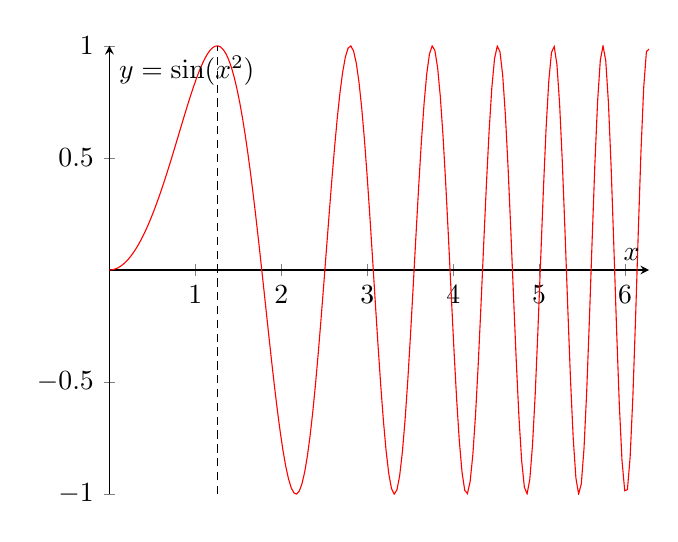
\begin{tikzpicture}
    \begin{axis}[
      axis lines = center,
      xlabel = $ x $,
      ylabel = {$ y = \sin(x^2) $},
      vasymptote = 1.2533141373155001
    ]
      \addplot[domain = 0:6.28, color = red, samples=200] {sin(deg(x^2))};
    \end{axis}
  \end{tikzpicture}}
\end{center}
Consider the function $ x \mapsto \sin (x^2) $. This function is made up of two
functions, applied one after the other:
\begin{displaymath}
  x \xmapsto{f} x^2 \xmapsto{g} \sin(x^2).
\end{displaymath}
We often notate this \textit{function composition} as $ g \circ f $ (note that we
evaluate from the right, so $ (g \circ f)(x) = g(f(x)) $).

Obviously the derivative of $ \sin(x^2) $ is not just $ \cos(2x) $, since the former
has a stationary point at $ x = \sqrt{\dfrac{\pi}{2}} $ but $ \cos(\sqrt{2\pi}) \neq 0 $. This
shows us that, in general, the derivative of a function composition is not simply the composition
of the derivatives.

In fact, it turns out that the derivative of $ f \circ g $ is $ g' (f' \circ g) $; in other words,
\begin{displaymath}
  \od{}{x} f(g(x)) = g'(x) f'(g(x)).
\end{displaymath}
This is known as the \textbf{chain rule}, since we are ``chaining" together functions.

Before proving the chain rule, let us convince ourselves that it is plausible. We can interpret the
derivative $ \od{g}{x} $ as the rate of change of $ g $ with respect to $ x $, and the derivative $ \od{f}{g} $
as the derivative of $ f $ with respect to small changes in $ g $; it is intuitive that if $ g $ changes
twice as fast as $ x $ at some point, and $ f $ changes five times as fast as $ g $, then $ f $ changes $ 2 \times 5 = 10 $
times as fast as $ x $.

The actual proof (given below) matches this intuition quite well.

\begin{exs}\leavevmode
  \begin{enumerate}
    \item The correct derivative of $ \sin(x^2) $ is $ 2x \cos(x^2) $.
    \item If $ f(r) = \sqrt{r^2 - 3} $, then $ f'(r) = 2r \frac{1}{2} \left(r^2 - 3\right)^{-1/2} = \dfrac{r}{\sqrt{r^2 - 3}} $.
    \item If $ g(x) = \sin((\sin^7 x^7 + 1)^7) $, then we compute:
          \begin{align*}
            g(x)  &= \sin \left( \left[ \left( \sin x^7 \right)^7 + 1 \right]^7 \right)\\
            g'(x) &= 7x^6 \cdot \cos x^7 \cdot 7\left(\sin x^7\right)^6 \cdot 7\left[\left(\sin x^7\right)^7 + 1\right]
                          \cdot \cos \left( \left[ \left( \sin x^7 \right)^7 + 1 \right]^7 \right)
          \end{align*}
          This result can probably be simplified, however the point is to evaluate the derivative chain from inside to outside in a systematic fashion.
  \end{enumerate}
\end{exs}

\begin{proof}[Proof of the chain rule (optional)]
  The proof is a little fiddly, and comes in two parts. Recall that in the work on limits, we found that an alternative definition of
  the derivative of $ f $ at $ x $ was
  \begin{displaymath}
    f'(x) = \lim_{k \to x} \frac{f(x) - f(k)}{x - k}.
  \end{displaymath}

  Now, suppose we wish to find the derivative of $ f \circ g $ at $ x $. In the first case, suppose that $ g $ is not constant
  around $ x $ (in other words, we can zoom in `far enough' towards $ x $ so that for all $ k $ in the zoomed in area, $ g(k) \neq g(x) $).
  Then:
  \begin{align*}
    \lim_{k \to x} \frac{f(g(x)) - f(g(k))}{x - k} &= \lim_{k \to x} \frac{f(g(x)) - f(g(k))}{g(x) - g(k)} \cdot \frac{g(x) - g(k)}{x - k}\\
                                                   &= \lim_{k \to x} \frac{f(g(x)) - f(g(k))}{g(x) - g(k)} \cdot \lim_{k \to x} \frac{g(x) - g(k)}{x - k}\\
                                                   &= f'(g(x)) g'(x),
  \end{align*}
  (noting that as $ k \to x $, $ g(k) \to g(x) $). This calculation only works when $ g $ is not constant around $ x $, because if $ g $ \emph{is}
  constant around $ x $ then for all $ k $ sufficiently close to $ x $, $ g(x) - g(k) = 0 $ and the limit does not exist.

  To deal with this case, assume that $ g $ \emph{is} constant around $ x $. Then $ g'(x) = 0 $, and also for all $ h $ close enough
  to zero we have $ g(x + h) = g(x) $. Then
  \begin{displaymath}
    (f \circ g)'(x) = \lim_{h \to 0} \frac{f(g(x + h)) - f(g(x))}{h} = \lim_{h \to 0} \frac{f(g(x)) - f(g(x))}{h} = 0 = 0 \times f'(g(x)) = g'(x) f'(g(x)).
  \end{displaymath}
\end{proof}

\clearpage
\subsection*{Questions}
\begin{questions}
  \questioA Identify the inner and outer functions, but do not attempt to differentiate.
    \begin{parts}
      \part $ \sqrt{\sin x} $
      \part $ \sin \cos \tan x $
      \part $ (2x + 3)^{17} $
      \part $ 97(x + 2)^2 $
      \part $ \ln \sin x $
      \part $ \frac{1}{\sqrt{23x - x^2}} $
    \end{parts}
  \questioA Differentiate with respect to $ t $:
    \begin{multicols}{2}
    \begin{parts}
      \part $ (2t + 3)^{3000} $
      \part $ \sin \ln t $
      \part $ \sqrt{t^3 + 10t^2 + 3} $
      \part $ \csc e^t $
      \part $ \sin^3 t + 14\ln (3t) $
      \part $ \sin \sin \sin t $
      \part $ \cot (t + \sec t) $
      \part $ \sin^2 ((t + \sin t)^2) $
      \part $ \ln \sqrt{t + 9} $
      \part $ \sqrt{t} + \frac{1}{\sqrt[3]{t^4}} $
      \part $ e^{\sec (t^2)} $
      \part $ \sin \sqrt{t + \tan t} $
    \end{parts}
    \end{multicols}
  \questioA The derivative of a function is $ 2 \cos 2x $. What could the original function be?
  \questioM Differentiate $ y = \sin^2 x + \cos^2 x $, and hence prove that $ \sin^2 x + \cos^2 x = 1 $.
  \questioA Suppose that the displacement of a particle on a vibrating spring is given by $ x(t) =  5 + \frac{1}{8} \sin(5\pi t) $,
            where $ x $ is measured in centimetres and $ t $ in seconds.
    \begin{parts}
      \part Find the velocity of the particle at time $ t $.
      \part At which times is the particle momentarily stationary?
    \end{parts}
  \question The volume of a spherical balloon at a time $ t $ is given by $ V(t) = \frac{4}{3} \pi r^2 $, and its radius, changing
            over time, is given by $ r(t) $. Find $ \od{V}{t} $ in terms of $ \od{r}{t} $.
  \questioM If $ F(x) = f(3f(4f(x))) $, where $ f(0) = 0 $ and $ f'(0) = 2 $, find $ F'(0) $.
  \questioA Suppose $ f(x) = g(x + g(a)) $ for some differentiable function $ g $ and constant $ a $. Find $ f'(x) $.
  \question The depth of water at the end of a jetty in a harbour varies with time due to the tides. The depth
            of the water is given by the formula
            \begin{displaymath}
              W = 4.5 - 1.2 \cos \frac{\pi t}{6}
            \end{displaymath}
            where $ W $ is the water depth in metres, and $ t $ is the time in hours after midnight.
    \begin{parts}
      \parA What is the rate of change of water depth 5 hours after midnight?
      \parM When is the first time after $ t = 0 $ that the tide changes direction?
      \parE At that time, is the water changing from rising to falling or from falling to rising?
    \end{parts}
  \questioM In physics, the rate of change of momentum of an object is proportional to the force needed to effect
            that change: if $ p $ is the momentum of the object as a function of time, $ F = \od{p}{t} $. The momentum
            of a particular object, oscillating back and forth along a line, is given by $ p = mA\sin(\omega t + \phi)\thinspace\si{\kilo\gram\metre\per\second} $
            (where $ m $, $ A $, $ \omega $, and $ \phi $ are various constants). What is the force acting on the object at $ t = 10 $?
  \question The force $ F $ (in newtons) acting at an angle $ \theta $ with the horizontal that is needed
            to drag a mass of $ W $ kilograms along a horizontal surface at a constant velocity is given by
            \begin{displaymath}
              F = \frac{\mu W}{\cos \theta + \mu \sin \theta}
            \end{displaymath}
            where $ \mu $ is the coefficient of static friction (a constant).
    \begin{parts}
      \parA If $ W = \SI{200}{\kilo\gram} $ and $ \mu = 0.2 $, find $ \od{F}{\theta} $ when $ \theta = \frac{\pi}{6}\thinspace\si{\radian} $.
      \parM Suppose now that $ \theta $ is a function of time, so that $ \od{\theta}{t} = \SI{0.5}{\radian / \second} $. Find $ \od{F}{t} $.
    \end{parts}
  \questioE Find the 73rd derivative of $ \sin 6x $.
  \questioE Recall that the \emph{absolute value} of $ x $, denoted $ \abs{x} $, is the value obtained by `throwing away the sign' of $ x $.
    \begin{parts}
      \part Prove that
            \begin{displaymath}
              \od{}{x} \abs{x} = \frac{x}{\abs{x}}.
            \end{displaymath}
            [\textit{Hint: Write $ \abs{x} = \sqrt{x^2} $.}]
      \part If $ f(x) = \abs{\sin x} $, find $ f'(x) $ and sketch the graphs of both $ f $ and $ f' $.
    \end{parts}
  \questioS In the next section, we will be studying the product rule for derivatives. It is possible, though not
            particularly usual, to prove it using simply the basic derivatives from the last section and the chain
            rule; in this exercise, you will do just that.

            Suppose that $ f $ and $ g $ are functions, and consider the function $ F $ defined by $ F(x) = \left(f(x) + g(x)\right)^2 $.
    \begin{parts}
      \part Calculate $ F'(x) $ using the chain rule.
      \part Calculate $ F'(x) $ by multiplying out the square and differentiating the polynomial that results. (In particular, note
            that $ \od{}{x} 2(fg)(x) = 2 (fg)'(x) $).
      \part Compare parts (a) and (b).
    \end{parts}
\end{questions}
\end{document}
